\documentclass[conference]{IEEEtran}
% Workshop-paper draft, Nov 2026. Numbers: results/retrain_nov2026 (docs/RESULTS_NOV2026.md);
% every prediction was registered first in docs/PREREGISTRATION_NOV2026.md.
% Build: cd paper/latex && pdflatex main && bibtex main && pdflatex main && pdflatex main
\usepackage[T1]{fontenc}
\usepackage[utf8]{inputenc}
\usepackage{amsmath,amssymb}
\usepackage{graphicx}
\usepackage{booktabs}
\usepackage{multirow}
\usepackage{xcolor}
\usepackage[hidelinks]{hyperref}
\graphicspath{{../figures/}}
\newcommand{\phiA}{\ensuremath{\phi}}

\begin{document}

\title{You Cannot See Grip Without Using It:\\Active Probing for Rapid Motor Adaptation in Autonomous Racing}

\author{\IEEEauthorblockN{Nathan Chong}
\IEEEauthorblockA{University of Hawai\textquoteleft i at M\={a}noa\\NSF REU, University of Nevada, Las Vegas}
\and
\IEEEauthorblockN{Venkata Prashant Modekurthy}
\IEEEauthorblockA{University of Nevada, Las Vegas}}

\maketitle

\begin{abstract}
Tire--road friction sets a race car's safe envelope, changes with surface and wear, and is not measured by any onboard sensor. Rapid Motor Adaptation (RMA) infers such hidden conditions from a robot's recent motion. Applied to grip on the F1TENTH platform, it cannot work as usually trained: with the car's actions decoupled from grip, its motion history carries no grip information ($R^2\!\approx\!0$ for three tire models), because the car is near neutral steer and drives inside the friction circle. Adaptation modules that appear to work instead read grip off the expert's own driving or simply drive slowly; a speed-capped non-adaptive car matches them. We add an \emph{active probe}, a brief speed pulse on straights that asks the tires for more than low grip can give. Grip becomes readable ($R^2$ 0.89--0.93), the car drives within 0.1\,m/s of an oracle at every grip, and at $\mu\!=\!0.4$ it crashes in 2--8\% of episodes versus 33--47\% for a non-adaptive car matched to its speed, on three training seeds; no fixed speed limit matches it on both speed and safety. Retrained with the car's real sensing (wheel odometry with slip, kinematic yaw rate, 40\,Hz LiDAR), a braking probe and a racing expert, the controller still reads grip ($R^2$ 0.84--0.87) and, at equal average speed, cuts crashes at $\mu\!=\!0.6$ from 33--56\% to 0--5\%. All hypotheses were pre-registered, including those that failed.
\end{abstract}

\section{Introduction}
Grip limits safe control, and it changes with rain, dust, tire wear and payload. A controller tuned for nominal grip is conservative everywhere or unsafe when grip falls. RMA~\cite{kumar2021rma} trains a base policy with privileged physics and an adaptation module that recovers those physics from recent states and actions; it works for legged robots and quadcopters~\cite{zhang2025extreme}, whose dynamics expose the hidden parameters continually.

A car's grip is different. Below the limit the tires deliver whatever force is asked, at any grip; grip shows only near the limit, which a cautious controller never visits. This is the familiar excitation requirement of tire--road friction estimation~\cite{acosta2017friction,khaleghian2017survey}. We ask whether an RMA controller on F1TENTH can infer grip from its own motion, and whether adapting to it beats simply driving slower.

\textbf{Contributions.}
(1)~A \emph{leakage-free observability test}: rolling out the policy with a random grip belief, independent of the true grip, removes the information the controller's own actions carry. Under it, the motion history contains no grip information, which explains why standard RMA fails here and why apparent successes are leakage.
(2)~\emph{Active grip probing} for RMA: a short speed pulse on straights, applied identically to all controllers, makes grip readable and yields oracle-like speed modulation.
(3)~A \emph{speed-matched control} that separates adaptation from slowness: without the probe, slowness explains all of the safety gain; with it, it does not.
(4)~Transfer to realistic car sensing, including a closed-loop check of the deployment node, and a robustness analysis of the wheel-slip assumption.
(5)~Pre-registered hypotheses with dated amendments, paired episodes, three training seeds and held-out tracks.

\section{Related Work}
\textbf{RMA} regresses an adaptation module onto privileged encodings and trains it on its own rollouts~\cite{kumar2021rma}; the quadcopter variant adds joint PPO and imitation~\cite{zhang2025extreme}. We show a second reason on-policy training matters: action leakage.
\textbf{Learning on F1TENTH} includes LiDAR-only deep RL~\cite{hell2024lidar,evans2023trajectory}, imitation benchmarks~\cite{sun2023ilbenchmark} and a survey~\cite{evans2024unifying}; none estimates physics online. RL racing policies have been deployed zero-shot on F1TENTH cars with domain randomization and actuator modeling~\cite{czechmanowski2025racing} and with disturbances and observation preprocessing~\cite{budai2025endtoend}. History-dependent policies help domain-randomized transfer~\cite{chen2022understanding,tobin2017dr}. The same group estimates velocity on F1TENTH with a learned dynamics model and an online friction estimate~\cite{wegrzynowski2024velocity}, and proposes long-horizon memory beyond RMA's short reactive window~\cite{czechmanowski_beyond}.
\textbf{Friction estimation} needs excitation: slip-based estimators need high tire utilization (up to 80--90\% on low-$\mu$ surfaces~\cite{acosta2017friction}; 54--94\% for a brush-model estimator~\cite{prokes2016excitation}) and fail in steady driving~\cite{khaleghian2017survey}. We bring this requirement to learned adaptation and meet it with a deliberate excitation.

\section{Method}
\textbf{Simulator.} f1tenth\_gym~\cite{okelly2020f1tenth} single-track model at 100\,Hz. Its tire is linear and never saturates, so we add a friction-circle tire: each axle's lateral force is capped at $\sqrt{(\mu F_z)^2-F_x^2}$ and acceleration at $\mu g$.
\textbf{Observation and action.} $x_t\in\mathbb{R}^{113}$: speed, steering, the previous speed and steering commands, yaw rate, and 108 LiDAR beams; action: steering and speed command (0--3\,m/s). No map or pose.
\textbf{Randomization.} Per episode, grip $\in[0.4,1]$ ($\mu=1.0489\cdot$grip); mass, inertia, steering and drive gains $\pm20\%$; actuator delays 0--50\,ms; mid-episode grip drops in 30\% of episodes; LiDAR noise and dropout.
\textbf{Phase 1.} Policy $\pi(x,z)$ (MLP $3\times256$) and encoder $z=\mu(e)\in\mathbb{R}^8$, trained by DAgger from a grip-aware Pure Pursuit expert~\cite{coulter1992purepursuit} on 13 scaled circuits~\cite{betz2022racing}.
\textbf{Phase 2.} \phiA{}: a 1-D CNN mapping the last 50 steps (0.5\,s) to $\hat z$, trained by regression on oracle-driven data and then three on-policy rounds~\cite{kumar2021rma}.
\textbf{Controllers.} One frozen $\pi$ with three sources of $z$: \emph{Oracle} $\mu(e_\text{true})$, \emph{\phiA{}} (estimated), \emph{Blind} $\mu(e_\text{nominal})$; plus Blind with a speed limit matched to \phiA{}'s measured speed.
\textbf{Active probe.} Every 0.5\,s on straights ($|\delta|<0.15$\,rad), the speed command is offset for 0.1\,s ($+2$\,m/s in configuration Q, $-1$\,m/s braking in R). The speed controller then requests more than $\mu g$ at low grip, so the response measures grip. The probe runs for every controller, in training and evaluation.
\textbf{Leakage-free test.} Roll out $\pi$ with a grip belief drawn independently of the true grip, so actions carry no grip information, and fit (i) a ridge probe on physical window features and (ii) \phiA{}'s network, cross-validated by episode.
\textbf{Evaluation.} $\mu\in\{1.0,0.8,0.6,0.4\}$, 100 episodes per cell from seeded random starts shared by all controllers (paired); exact McNemar tests on paired crashes, Holm-corrected; E5: grip $R^2$ of $\hat z$ over 200 episodes.

\section{Results}
\subsection{Without excitation, grip is not observable}
With grip-independent driving, physical features of 0.5\,s windows predict grip with $R^2\!=\!-0.02$ (friction-circle tire) and $-0.03$ (Fiala brush tire); with oracle or \phiA{}-driven data they reach 0.97 and 0.68, all of it leakage. Below the limit, grip barely changes the yaw response ($-3\%$ to $-5\%$ at 1.5--2\,m/s, $\mu$ 0.4 vs 1.0), and the policy's 99th-percentile accelerations (3--3.7\,m/s$^2$ longitudinal, $\sim$2\,m/s$^2$ lateral) stay under even low-grip $\mu g$. With the probe, the same test gives $R^2\!=\!0.84$; \phiA{}'s network learns it from proprioception (0.67) but not from all 115 channels (0.15).

Standard RMA fails accordingly. Trained on oracle-driven data, \phiA{} drives faster than the oracle at every grip and crashes more than Blind at $\mu\!=\!0.4$ (0.39 vs 0.32). Trained on its own rollouts with the friction-circle tire, \phiA{} is far safer than Blind (0.04 vs 0.44) but slows only 0.10--0.19\,m/s with grip ($R^2$ 0.28), and Blind capped at \phiA{}'s speed is as safe on every seed.

\subsection{With the probe, adaptation beats a speed limit}
\begin{table}[t]
\centering
\caption{Configuration Q (ideal sensors + probe), per training seed. N\,=\,100 paired episodes per cell.}
\label{tab:q}
\begin{tabular}{@{}lccc@{}}
\toprule
 & seed 0 & seed 1 & seed 2\\
\midrule
\phiA{} speed, $\mu$ 1.0$\to$0.4 (m/s) & 2.02$\to$1.28 & 2.06$\to$1.29 & 2.00$\to$1.28\\
Oracle speed, $\mu$ 1.0$\to$0.4 & 2.12$\to$1.27 & 2.11$\to$1.27 & 2.11$\to$1.26\\
Crash $\mu$\,0.4: \phiA{} / Blind & 0.07 / 0.46 & 0.02 / 0.47 & 0.08 / 0.43\\
Speed-matched Blind, $\mu$\,0.4 & 0.37 & 0.47 & 0.33\\
\quad McNemar $p$ vs \phiA{} & $2\!\times\!10^{-9}$ & $6\!\times\!10^{-14}$ & $6\!\times\!10^{-8}$\\
E5 grip $R^2$ & 0.90 & 0.93 & 0.89\\
\bottomrule
\end{tabular}
\end{table}

\begin{figure}[t]
\centering
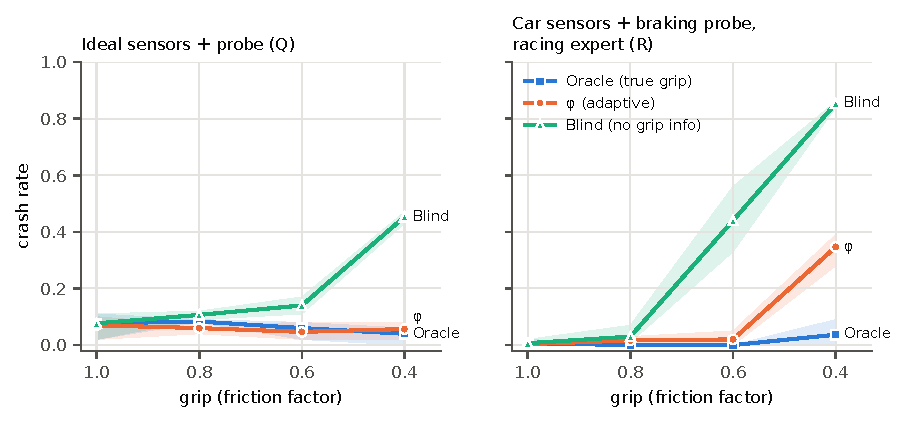
\includegraphics[width=\columnwidth]{fig1_crash_vs_grip.pdf}
\caption{Crash rate vs.\ grip for the same base policy with the true grip (Oracle), \phiA{}'s estimate, or none (Blind). Mean of 3 training seeds (band: min--max), N\,=\,100 paired episodes per point. Left: ideal sensors; right: car sensors, braking probe and racing expert.}
\label{fig:crash}
\end{figure}

Table~\ref{tab:q} and Fig.~\ref{fig:crash} (left) show configuration Q. \phiA{} reads grip ($R^2$ 0.89--0.93), drives within 0.1\,m/s of the Oracle at every grip, and is as safe as the Oracle. Because the probe adds speed on top of a limit, the matched Blind is capped so its \emph{measured} speed equals \phiA{}'s; it still crashes 5--20 times as often at $\mu\!=\!0.4$. A sweep of fixed limits (Fig.~\ref{fig:frontier}) shows that matching \phiA{}'s safety costs 19--29\% speed on full grip. With the probe switched off at test time, the same \phiA{} falls back to a constant $\sim$1.2\,m/s ($R^2$ 0.24); on three held-out tracks a model that never saw them closes 80\% of the Oracle gap (87\% for one trained on them); after a grip drop the estimate settles in 0.77\,s. The probe changes Blind's and the Oracle's crash rates by at most 0.02.

\begin{figure}[t]
\centering
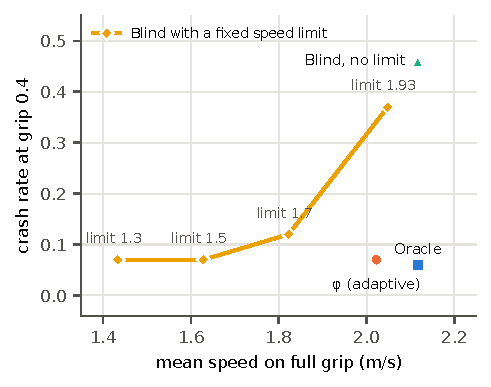
\includegraphics[width=0.85\columnwidth]{fig2_frontier.pdf}
\caption{Speed on full grip vs.\ crash rate at $\mu\!=\!0.4$ (seed 0, Q). A fixed speed limit trades one for the other; \phiA{} gets both. Lower right is better.}
\label{fig:frontier}
\end{figure}

\subsection{Realistic car sensing and racing speed (R)}
Configuration R builds the observation the way the car's node builds it from the standard F1TENTH stack: speed from VESC wheel odometry (the wheel spins up or locks when traction-limited; $\pm5\%$ gain error; 50\,Hz), yaw rate computed as $v\tan\delta_\text{cmd}/L$ (no gyro), commanded steering, and 40\,Hz LiDAR. The probe is a braking pulse (an accelerating one asked for 5\,m/s before corners), \phiA{} also sees ten front LiDAR beams, and the expert races: full speed on straights, corners at $\sqrt{0.6\mu gR}$. Base policies are faster and safer (2/117 validation crashes at $\sim$2.5\,m/s, vs 3/39 at 1.2--2.0\,m/s).

\phiA{} still reads grip ($R^2$ 0.84--0.87). All three controllers drive at about the same average speed; adaptation is \emph{where} to slow (Fig.~\ref{fig:crash}, right). At $\mu\!=\!0.6$, \phiA{} crashes 0--5\% vs 33--56\% for Blind (Oracle 0\%); at $\mu\!=\!0.4$, 28--39\% vs 84--86\% (Oracle 0--9\%), and Blind matched to \phiA{}'s measured speed crashes 84--86\% ($p<10^{-13}$, every seed). The pre-registered checks pass on every seed, except a ratio of cross-grip variance that even the Oracle fails with the probe.

\subsection{Robustness to the wheel-slip model}
\begin{figure}[t]
\centering
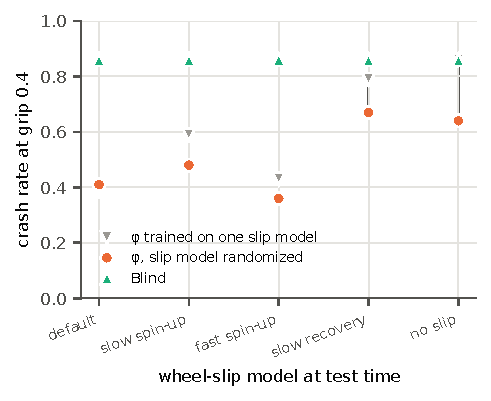
\includegraphics[width=0.85\columnwidth]{fig4_slip.pdf}
\caption{Crash rate at $\mu\!=\!0.4$ under five wheel-slip models at test time (seed 0, R). \phiA{} trained on one slip model is blind without slip; randomizing the slip model in training removes this.}
\label{fig:slip}
\end{figure}

The wheel-slip model is an assumption. Evaluated under four alternatives, \phiA{} degraded and, with no slip at all, was blind (Fig.~\ref{fig:slip}; $\mu\!=\!0.4$: 0.86 vs 0.86 for Blind), although the true deceleration and the front LiDAR still carry the information. Retraining \phiA{} with the slip model randomized per episode costs nothing under the default model and beats Blind in all 30 slip-model $\times$ seed $\times$ grip comparisons ($\mu\!=\!0.6$: $\le$0.07 vs 0.29--0.56); with no slip it reads grip at $R^2$ 0.59--0.63 (Fig.~\ref{fig:readability}). The pre-registered margin at $\mu\!=\!0.4$ (0.30) is missed on one seed for the two weakest-signal models (0.19, 0.22).

\begin{figure}[t]
\centering
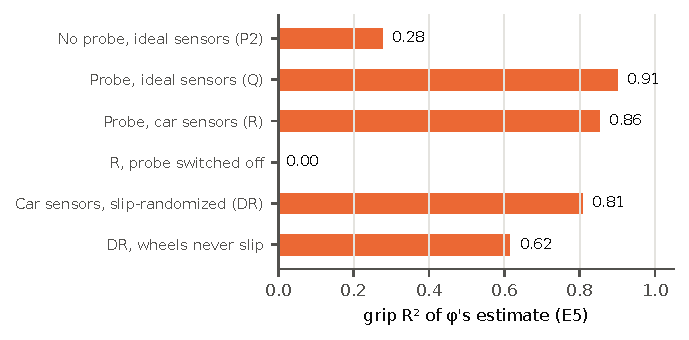
\includegraphics[width=0.85\columnwidth]{fig3_readability.pdf}
\caption{Grip $R^2$ of \phiA{}'s estimate (E5) by configuration; mean over training seeds where available.}
\label{fig:readability}
\end{figure}

\subsection{Real-car pilot}
In July, an F1TENTH car (Traxxas Slash 4$\times$4) ran an earlier checkpoint (linear tire, no probe, and a 50\,Hz node against 100\,Hz training) through one 90$^\circ$ corner with four tire wraps (81 trials); its steering and yaw rate differed between bare and electrical-tape tires (uncorrected $p\!=\!0.0001$ and $0.009$; over the nine comparisons the analysis runs, steering survives a Bonferroni--Holm correction and yaw does not; effects of $-3.8\%$ and $-2.5\%$). This shows the policy responds to a real tire change, not that the probe works on the car.

\section{Discussion and Limitations}
\textbf{The probe changes the method:} the controller spends a small, fixed amount of driving on measurement; a learned, risk-aware probing policy is future work.
\textbf{The wheel-slip model is assumed}, and the controller is strongest when its signature is present. A one-session test measures it: braking pulses on three surfaces, logging odometry, IMU and front-LiDAR range; a simulated version of the test predicts that odometry alone separates grip 1.0/0.7/0.4 ($p<10^{-7}$).
\textbf{At $\mu\!=\!0.4$ a gap remains} under realistic sensing (49--58\% of the Oracle gap closed vs 82--87\% with ideal sensors), plausibly because the estimate depends on probes on straights.
\textbf{Regime:} speeds $\le$3\,m/s on narrow scaled tracks, uniform grip, simulation only for every probe result.

\section{Conclusion}
On F1TENTH, RMA cannot infer grip from passive driving: the information is not in the motion, and adaptation modules that appear to succeed are reading their own actions or driving slowly. A brief, deliberate probe makes grip observable; with it, an RMA controller matches an oracle's speed at every grip and beats any fixed speed limit at low grip, across seeds, held-out tracks and realistic car sensing. Whether the real car's wheels reveal grip under a braking pulse as the model assumes is the next, one-session experiment.

\section*{Acknowledgment}
Supported by NSF REU Site Award \#2349616 (UNLV Smart Cities). Thanks to Ederic Oytas for hardware support.

\bibliographystyle{IEEEtran}
\bibliography{../references}

\end{document}
